%This is a LaTeX template for homework assignments
\documentclass{article}
\usepackage[utf8]{inputenc}
\usepackage{amsmath, pgfplots, mathtools}
\pgfplotsset{compat=1.14}

\begin{document}
\title{Section 3.1 Review Worksheet}

\section*{Section 3.1 Review} %Assignment Title
Name: \line(1,0){120} %you can change the length of the lines by changing the number in the curly brackets
\\Date: \line(1,0){125}

%\subsection*{Instructions} %Instruction Title
%Please solve these equations by graphing.

\subsection*{Section A}
Please use substitution to determine if the given ordered pair is an element of the solution set for the systems of equations.
\begin{enumerate}%starts the numbering

\item $(1,7);$
	$\begin{cases}
		y=2x+5 \\ y=3x-5
	\end{cases}$
\item $(-1,-7);$
	$\begin{cases}
		-x+y=-6 \\ -5x+y=-2
	\end{cases}$

% \item Evaluate the following integral 
% \begin{equation*}
% \int_{2}^{x} \sinh{2y}\, \mathrm{d}y
% \end{equation*}
% in the case where:
%     \begin{enumerate}
%     \item $x = 5$
%     \\\line(1,0){250}
%     \\\line(1,0){250}
%     \\\line(1,0){250}
%     \item $x = 9$
%     \\\line(1,0){250}
%     \\\line(1,0){250}
%     \\\line(1,0){250}
%     \end{enumerate}
    
% \item Find the determinant of the following 3x3 matrix:
% \begin{figure}[h!]%This example matrix has been enclosed in a figure to give us more positioning options
% \centering
% \begin{math}
% \begin{pmatrix}
% 1 & 6 & 4 \\
% 3 & 1 & 7 \\
% 9 & 4 & 5
% \end{pmatrix}
% \end{math}
% \end{figure}
% \\\line(1,0){300}
% \\\line(1,0){300}
% \\\line(1,0){300}

\end{enumerate}%ends the numbering

\subsection*{Section B}
Use a graph and a table to solve the system.
% \begin{enumerate}

% \item Determine the following limit:
% \begin{equation*}
% \lim_{x \to +\infty} \frac{\sin{x}}{x^2}
% \end{equation*}
% \\\line(1,0){300}
% \\\line(1,0){300}
% \\\line(1,0){300}

% \item Describe the Gram-Schmidt Algorithm.
% \\\line(1,0){300}
% \\\line(1,0){300}
% \\\line(1,0){300}

% \end{enumerate}
\begin{enumerate}
\item $\begin{cases}
	y=3x+4 \\ 3x+2y=5
\end{cases}$
\begin{figure}[h!]
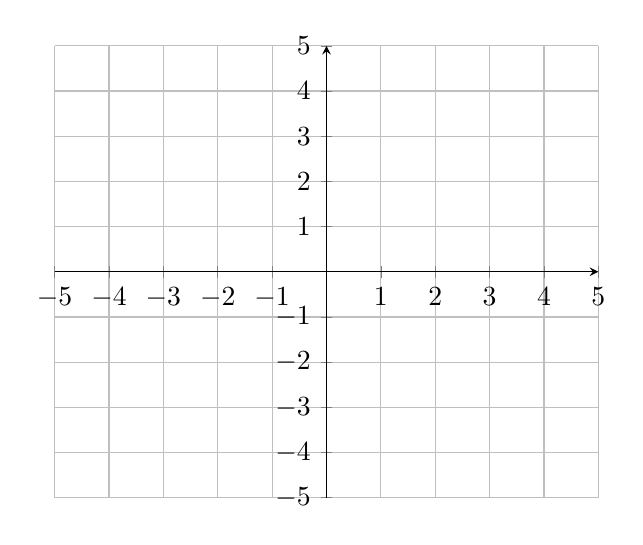
\begin{tikzpicture}
  \begin{axis}[
    width=0.7\linewidth,
    axis lines=middle,
    grid,
    ymin=-5,
    ymax=5,
    ytick={-5,...,5},
    xmin=-5,
    xmax=5,
    xtick={-5,...,5},
    %xticklabel={\pgfmathprintnumber{\tick}:00},
    %xticklabel style={rotate=45,anchor=north east}
    ]
  \addplot[draw=none] coordinates {(1,1)};
  \end{axis}
\end{tikzpicture}
\end{figure}
\end{enumerate}

\subsection*{Section C}
Use a graph and a table to solve the system.  Use your calculator.
\begin{enumerate}
\item
	$
  \begin{cases}
    	y=3 \\
      	3x+8y=28
  \end{cases}
	$
\end{enumerate}
\end{document}